\documentclass[a4paper]{article}
\newtheorem{hyp}{Hypothesis}
\usepackage{graphicx}
\graphicspath{ {/home/angelo/Documents/Uni/Courses/Data Managment & Ethics/Integrated Assignment/assignemnet_project_folder/ERDs/} }


\begin{document}

\title{DME Integrative Assignment}
\author{Angelo Barisano; 508903 }
\date{September 16th, 2022}
\maketitle

\newpage
\section{Task 1: Plan \& Explore}

\subsection{Origin of Data \& Purpose Introduction}
\paragraph{Introduction} Data drives security. The wide spread adoption of data information systems has been used to recognize crime hot-spots to increase policing efficiency and protect people. Thus, creating effective information systems for crime prevention is at the center of policy makers and executive branches of governments. This trend has led to the Chicago PD reaching out to this data management team with the request of creating a Data Management System for crime-data in Chicago.

To this end, the Chicago PD and this Data Management Unit is interested on setting the foundation for a FAIR database to answer research questions; i.e. a data base meant to flexible and easy in use of slicing and dicing data to find answers and, contemporaneously, make them available. Additionally, any code produced during this endeavour will be made public on GitHub for transparency purposes. 

\paragraph{Data Description in Scope, Volume, and Format}
The data was provided by the Chicago PD contains a sample of 730,900 registered crimes in the administrative districts of Chicago between the years of 2017 and 2021. The initial data source is in CVS-format and pertains to specific recorded crimes in the administrative jurisdiction of the Chicago PD in addition to time, location, crime type, and arrested or not. Thus, the data contact is to be found on the Chicago PD website (\textbf{CITE THE CHICAGO WEBSITE FOR THE DATA}). Considerations regarding the ethical (\& GDPR compliant regardless of whether the data comes from the USA) use of the data will be discussed in part 5 of this assignment.

\paragraph{Project time frame, researchers, and misc information} The set project time frame is the 27th of August 2022 till 2nd of October 2022. Involved in this project is only one student, Angelo Barisano. Additionally, this project is designed to comply with FAIR standards (\textbf{CITE FAIR STUFF HERE}).

\subsection{WHAT IS THE PURPOSE OF THIS ASSIGNMENT??}

\subsection{Research Question}

\textbf{In an iterative (agile) development cylce the following questions have been set up: Chicago is known for its high homicide rate; this leads to policy makers focusing on this issue the most. }

Upon conducting an initial Exploratory Data Analysis (EDA), three major categories were identified in the data: 

\begin{itemize}
  \item Location
  \item Crime type
  \item Crime record data (time, arrest, etc.)
\end{itemize}

Based on the data categories and EDA, the following research questions guide the creation of the database in increasing complexity. 

\paragraph{Question 1} Finding prevalent crime patterns in the data is a common starting point. Thus, this question provides future research with an adjustable query to gain an overview over the general distribution of crime by type. Subsequently applying a temporal component (i.e. by day of week,  month, year, season, etc.) to this initial distribution reveals trends and temporal patters. This way, this question helps to answer questions to policy makers regarding general trends; such as how crime developed overall and by type. As such:

\begin{itemize}
  \item How do crime types (e.g. homicides) patterns distributed by a temporal component? How do certain crime types (homicide) patterns distribute by seasonality patterns, by time of day?
\end{itemize}

\paragraph{Question 2} The next logical progression is to observe the location and crime dimension together. The assumption is that certain districts and beats tend to be more prevalent in certain crime types. Thus, question two follows:

\begin{itemize}
  \item Do certain crime patterns (e.g. for homicides) persist by location such as certain districts/ beats/ blocks?
\end{itemize}

\paragraph{Question 3}Finally, time, location, and crime type is triangulated. This enables policymakers to discern localized trends in the data in order to address crime patterns by distributing resources more efficiently; i.e. allocating more resources to dangerous beats during the night. Additionally, accessory dimensions will be integrated into the analysis to provide a holistic description. For instance assuming that crimes that lead to more arrests are more resource intensive, these crimes put a disproportionate strain on law enforcement. Thus, by triangulating arrests by location and e.g. time of day this will enable us to show areas that need more attention by law enforcement. Another angle would be a specific analysis of beats. \textbf{Beats are the smallest administrative unit of a police district; a beat is patrolled for one year by one unit and ten transferred to another beat. Thus, it might be interesting to investigate the connection between a subset of beats that suddenly stop showing problems during one year and then re-appear in terms of crime in another year. The sub-question would, thus, investigate whether beats that usually persisted in crime only persist on a closed yearly basis. This way, effective police units might be identified and resources might be allocated more efficiently.}
 
\begin{itemize}
  \item Triangulating time, crime-type, and location which areas persists in certain crimes wrt. time?
In order to prevent homicides; which “beats“ are the most prevalent among homicides? During which time of day (for effective allocation of policing resources)? 
\end{itemize}

As such, the final question considers a variety of hypotheses that can be explored. Overall, these project based questions are constructed in such a way that they guide an external user (PD) through the process of finding areas that need successively complex "sliced \& diced" information and culminate in the creation of actionable policy implications regarding prime prevention through resource allocation.


\textbf{ADD PLOTS of EDA ALREADY HERE!!!}


\section{Design and Organize}

\textbf{IMPORTANT!!!! READ THE DEFINITION FOR 3rd NF AGAIN; MAYBE CRIME AND LOCATION QUALIFY TO BE 3rd NF... but maybe also not. STRESS AGAIN THAT THE INCLUSION OF BLOCK IS NOT NEEDED FOR THIS RESEARCH!!!}

\paragraph{Entity 1: Case} Part 1 identified three relevant data categories.  The first component consist of the individual instances of cases. Conceptually, these are central to this project as they enable the creation of the frequency distributions conditional on time and/or location. The variables that define this entity are as follows:

\begin{itemize}
  \item CaseId
  \item DateTime object implicitly containing day, month, year, and time of day 
  \item Arrest Boolean  
´  \item \textbf{Location Description???????????????????????????????????????????}
\item \textbf{Location Description???????????????????????????????????????????}
\item \textbf{Location Description???????????????????????????????????????????}?????????????????????????????????????????????????????
\end{itemize}
 
The DateTime object will enable the clustering of crimes by the time dimension. Additionally, arrest information is used to further drill down the analysis and dissect the cases for more resource intensive cases. Finally, the dimensions of Latitude and Longitude will be included on the case level. The reason for this is, while lat-lon information pertains to the location category, this variable(s) is case specific due to its precision. Imagine the database where latitude and longitude would be described as a standalone entity hierarchically below district or beat. To make the relation work each location would have to carry a CaseId as a foreign key in order to identify what type of crime was perpetrated at this location. Assuming that the lat-lon information is sufficiently granular, this would create a one-to-one relationship between case and the lat-lon entity (disregarding district in this case). Any one-to-one relationship is redundant. Thus, it does not make sense to place lat-lon as a standalone entity hierarchically below district. The reason for the inclusion of lat-lon is its usage as geopandas objects in plotting crime in a heat-map in part 6. Please note that while the information of lat-lon technically violates 1st NF requirements, this information is not supposed to be processed via SQL (except for PostGIS applications) but as a datatype in scripting languages; thus it is an atomic item.

\textbf{The primary benefit of case as an entity is to make the following two dimensions compliant to the 2nd normal form (and to some extend compliant with 3rd normal form with some caveats) by default. If we were to leave out case as an entity and immediately match crime types and location, the resulting two entities could not comply with 3rd normal form as crime types and location (as categories) would produce a many-to-many relationship. As such, the case entity inadvertently functions as an associative entity, reducing many-to-many relationships to two many-to-one relationships.\footnote{I will not further elaborate on this; this is a logical conclusion; in order to reach 2nd normal form this is a required step which is obvious} As a consequence, case complies to the 3rd NF by definition as no stand alone entities are to be found in this entity, while requiring the other data categories to normalize as well. It is notable, that while such design choices should be reflected by leaving out case as an entity in the conceptual model in part 3 and then include it as part of the logical model, but case is so pivotal to the functioning of the database in its purpose, that we will consider it along the way a a valid entity.}

\paragraph{Entity 2: Crime Type} Every Case requires a crime to be a valid instance. The raw data provides the IUCR, which identifies each unique combination of primary (e.g. homicide) and secondary crime category (e.g. first degree). Generally, most headlines only consider the primary type of crime, such as homicides, and generally disregard the secondary description of the data, such as first, second, or third degree in this case \textbf{CITE SOME EXAMPLE NEWSPAPERS}. However, while this assignment might not need the information regarding secondary description; it is also the task of a FAIR database to enable future users to differentiate between different types of general crimes. Furthermore, it might be the case, that certain subcategories of crimes tend to be more prevalent than others. As such, the crime type entity contains both the primary category and the secondary description of the crime committed. It is notable that it does not make sense to further normalize this category, as the primary type column, though repeating, would be an entity of one dimension; thus, superfluous. \textbf{It is notable that the secondary description, while unique to the IUCR in most cases does not suffice to be the primary key due to some duplication (not unique) in addition to being long for some crime types.}


\paragraph{Entity 3 \& 4: Location} 
The first entity identified in this case pertains to (police) district. Following hierarchically, beats are below district; one district containing multiple beats. Thus, a natural hierarchy is being identified, resolving any issues regarding normalization when connecting case to district and then to beat. 

\textbf{It is notable, that the choice of splitting district from beat is a design choice meant to improve clarity and demonstrate knowledge of the 3rd NF. The existstence of beat as an entity technically removes the need for a district entity due to all information being included in the case and beat entity at the same time. If we were to remove the leation from district to case, the resulting queries would be more complex than needed.
MAYBE WE SHOULD REMOVE THE CONNECTION OF DISTRICT AND CASE!!!}

The reason to exclude block as a entity of analysis is threefold. 1) blocks overlap to some extend with different districts and beats increasing the level of analysis unnecessarily. 2) Beats and districts are administrative units, while blocks require local knowledge. 3) The information regarding the location of the case happening is already included in the lat-lon information in entitiy one as block only pertains to a reducted version of the address making the lat-lon information more informative when plotted (also: no map regarding blocks in chicago is available). 

\paragraph{Logging \& Master Table} Finally, a small master table will be included which tracks any information regarding formatting the data, data retrieval, and restrictions/ triggers called (not included in part 3 due to relevancy).


\paragraph{Conclusion} Due to the fundamental nature of the data, with the case itself being fundamental to the entire structure, all issues regarding normalization and inadvertently many-to-many relationships are solved as will be demonstrated in the next section.


\textbf{VERY IMPORTNAT: regarding the crime type YOU CAN USE THE PRIMARY TYPE AND SECONDARY TYPE BOTH TOGETHER IN ONE TABLE USING IUCR IN THE CRIME - THEN YOU CAN SIMPLY USE THE DESCRIPTION FOR ONE INTERESTING QUESTION AND ARGUE THAT THIS IS LEFT OVER SO THAT PEOPLE CAN DISTINUGSH FURTHER LATER DOWN}

\section{Part 3: ERD}

\textbf{IMPORTANT!!!!! DESCRIBE IN THE CONCEPTUAL MODEL ETC WITH TEXT THAT EG CRIME TYPE "HAS MANY" CASES ABOVE THE LINES LIKE ON THE SLIDES}

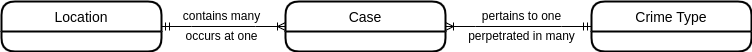
\includegraphics[scale=.35 ]{ConceptualDiagramFinal.drawiowdescription.png}

\subsection{Conceptual Model}
As mentioned in part 2, the individual case instance is central to the database design. Contemporaneously, the case entity resolves all problems regarding normal form and many-to-many relationships. Subsequently, the conceptual model describes the relation of the three entities described in part 2: 

\begin{itemize}
  \item Location
  \item Case
  \item Crime Type
\end{itemize}

\indent As can be seen in Figure 1, Location contains polygon information regarding where which administrative area the crime instance allocated to. Location is related to case utilizing beat as a foreign key in case (see Figure 3). This necessitates that this relation is directional from location to case; i.e. in one beat one or many cases can be instantiated. However, one case can only relate to one beat and district.

\textbf{INTERMEZZO It may be notable that the model shows mandatory relationships for Crime Type and location. Technically correct would be to use non mandatory relationships for location and crime type. For example a district or crime may not have been perpetrated and, thus, would not have a record. This research does not consider this case as the goal of this data base is to use the existing data for analysis. As such, in order for a district/ crime to be included in the database, a crime instance must have been created for these instances. As such, the choice was made to include a mandatory relationship.}

Following, case is related to crime type. Crime type describes the crime perpetrated. This is why, the IUCR is included as a foreign key in case. Consequently, the cardinality reads as one case only pertaining to one crime type being perpetrated. Contrarily, one crime type can be represented in many cases.

\subsection{Logical Model}
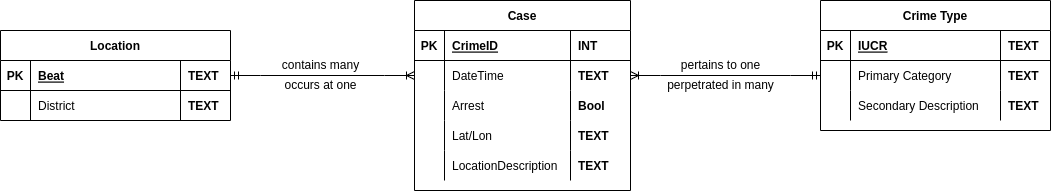
\includegraphics[scale=.35 ]{LogicalDiagramFinal.drawiowdescription.png}


Figure 2 describes the logical model. For location, "beat" is chosen as primary key because if we were to normalize this relation to 3rd NF, beat (as an entity) would be hierarchically below District; one district - many beats. As such, each district is uniquely identifiable by its beat in case we want to aggregate, which is why beat is the most suitable primary key. As argued in part 2, there is no reason to normalize to 3rd NF in this case. More importantly, the primary key beat is in TEXT form. The reason for this is that beats are defined in the first two characters by their district and the latter two describe the beat. Thus, a beat instance may start with a "0". In many scripting languages and some databases, this leads to problems and the removal of the "0", as the underlying software does not interpret the "0". As such, TEXT was chosen for data quality reasons. Please note that the same argument applies to crime type and IUCR. 
\indent Following, CrimeID was chosen to be the primary key of case, due to it being a natural primary key. This is a standard auto-incremental integer key and can, thus, be treated as an integer; though care should be applied when reading the data into scripting languages.
\indent Finally, crime type's primary key is the IUCR key, a natural primary key. It uniquely identifies each crime category plus its secondary description. 

\subsection{Physical Model}
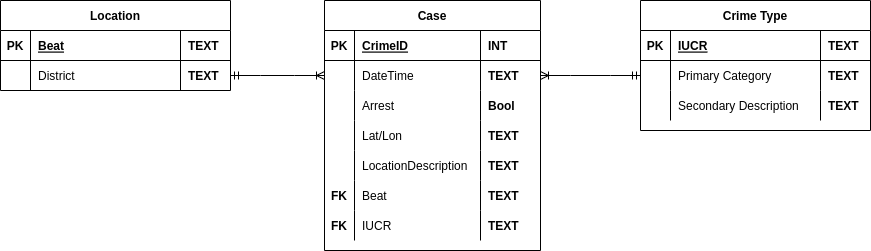
\includegraphics[scale=.35 ]{PhysicalModelFinal.drawio.png}

As mentioned in part 2, the inclusion of case as a full entity throught the entire process automatically removes any many-to-many relationships. Moreover, the usage of the appropriate foreign keys was discussed in section 3.1 in accordance to the cardinalities. As such, the logical model described in section 3.2 also corresponds to the physical model by definition with the exception of the foreign keys. The choice of foreign keys was made due to the direction of the cardinalities in Figure 3; beat and IUCR are natural keys for their respective entities and are, thus, unique.



\section{Part 4- Data Quality checks and preparation}


DATA TRIANGLE in lecture!!!
ALSO THE META DATA AND ETHICAL CONSIDERATIONS!! REGARDING GDPR that data quality is important to be complied by!!! This is also important for fair wrt interpretability and reusablity


Dropping instances
- remove all instances that do not have a casenumber - resulting in 3 instances removed from the database
- This returns another 79 porblematic instances where beat and district do not correspond
-an additional 16 entries do not contain dates; this is pivotal so they have to be removed


\section{Part 5}
ENCRYPTION OF DATABASE!!!!!!!!





\section{Part 6}
IMPORTANT! READ DATABASE INTO PYTHON HERE LIKE YOU DID AT VYTAL!!!







\end{document}
